\section{Zielsetzung}
\label{sec:Zielsetzung}

Mit dem Millikan-Versuch soll die Elementarladung $e_0$ bestimmt werden.
Dies wird durch die Messung der Gleichgewichts-, Sink- und Steiggeschwindigkeit von Öltröpfchen in einem elektrischen Feld erreicht.
Außerdem soll die Avogadro-Konstante $N_A$ bestimmt werden.

\section{Theorie}
\label{sec:Theorie}

Zur Versuchsdurchführung werden Tröpfchen durch Zerstäuben von Öl in eine Kammer gebracht.
Durch die Reibung bei der Zerstäubung werden die Tröpfchen elektrisch geladen.
Die Ladung der Tröpfchen beträgt immer ein ganzzahliges Vielfaches der Elementarladung $e_0$.

\subsection{Wirkende Kräfte}%Vielleicht lösche ich noch alle Überschriften
\label{sec:Wirkende Kräfte}

Auf die Tröpfchen wirken bevor eine Spannung an den Kondensator angelegt wird die Gravitationskraft $\vec{F_g} = m \vec{g}$ und die Stokesche Reibungskraft $\vec{F_R} = -6\pi r \eta_{\text{Lu}} \vec{v}$.
Dabei ist $m$ die Masse des Tröpfchens, $g$ die Erdbeschleunigung, $r$ der Radius des Tröpfchens, $\eta_{\text{Lu}}$ die Viskosität der Luft und $\vec{v}$ die Geschwindigkeit des Tröpfchens.
Die Stokesche Reibungskraft wirkt der Bewegungsrichtung entgegen.
Nach kurzer zeit stellt sich eine Gleichgewichtsgeschwindigkeit $v_0$ ein, bei der die beiden Kräfte gleich groß sind.
Die Tröpfchen erfahren verschwindent geringen Auftrieb, da die Dichte der Luft $\rho_{\text{Lu}}$ sehr gering ist.
Zur vollständigen Beschreibung der Gravitationskraft wird die Dichte der Luft dennoch mit angegeben.
Das Kräftegleichgewicht lautet
\begin{equation*}
    \frac{4 \pi}{3}r^3 \left(\rho_{\text{Öl}} - \rho_{\text{Lu}}\right) g = 6 \pi r \eta_{\text{Lu}} v_0 \, .
\end{equation*}
%Der folgende Absatz sollte vielleicht nochmal überarbeitet werden:
Wobei die Masse $m$ durch Masse $=$ Volumen $\cdot$ Dichte mit $\rho_{\text{Öl}} = \SI{886}{kg}$ als Dichte des Öls ersetzt wird. 
Durch auflösen nach $r$ ergibt sich der Radius des Tröpfchens zu
\begin{equation*}
    r = \sqrt{\frac{9 \eta_{\text{Lu}} v_0}{2 g \left(\rho_{\text{Öl}} - \rho_{\text{Lu}}\right)}} \, .
\end{equation*}

\subsection{Kräfte bei angeschaltetem Kondensator}
\label{sec:Kräfte bei angeschaltetem Kondensator}

%Die Grafik muss vielleicht noch verschoben werden um sinnvoller platziert zu sein:
\begin{figure}[H]
    \centering
    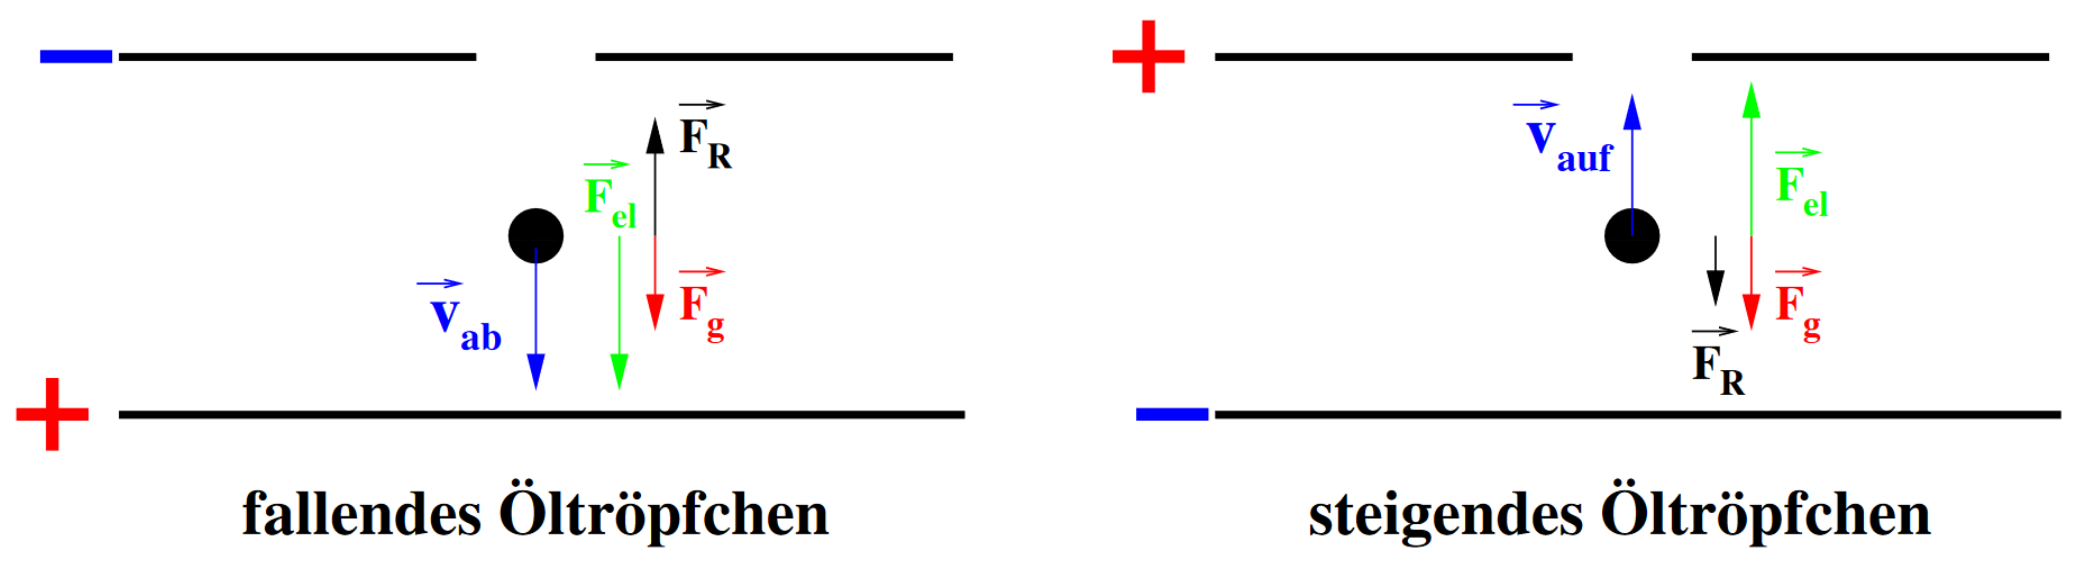
\includegraphics[width=0.7\textwidth]{img/kraefte.png}
    \caption{Wirkende Kräfte im angeschalteten Kondensator. \cite{V503}}
    \label{fig:Gleichgewichtskraefte}
\end{figure}

Wird nun eine Spannung $U$ an den Kondensator angelegt, wirkt zusätzlich die elektrische Kraft $\vec{F_{el}} = q \vec{E}$ auf das Tröpfchen.
Wie in \autoref{fig:Gleichgewichtskraefte} zu sehen ist, wird zwischen zwei Fällen unterschieden.
Im ersten Fall wirkt die elektrische Kraft in die gleiche Richtung wie die Gravitationskraft.
Das Tröpfchen bewegt sich kurz nach anlegen der Spannung mit einer konstanten Geschwindigkeit $v_{\text{ab}}$ in Richtung der unteren Platte.
Die Geschwindigkeit $v_{\text{ab}}$ ist dabei größer als die Gleichgewichtsgeschwindigkeit $v_0$.
Es stellt sich erneut ein Kräftegleichgewicht ein, welches durch
\begin{equation}\label{eq:v_ab}
    \frac{4 \pi}{3}r^3 \left(\rho_{\text{Öl}} - \rho_{\text{Lu}}\right) g - 6 \pi r \eta_{\text{Lu}} v_0 \, = -q\vec{E}
\end{equation} 
beschrieben wird.
Im anderen Fall wirkt $\vec{F}_e$ entgegen $\vec{F}_g$.
Die elektrische Kraft ist in diesem Fall größer als die Gravitationskraft.
Das Tröpfchen bewegt sich mit einer konstanten Geschwindigkeit $v_{\text{auf}}$ in Richtung der oberen Platte.
Hier stellt sich das Kräftegleichgewicht
\begin{equation}\label{eq:v_auf}
    \frac{4 \pi}{3}r^3 \left(\rho_{\text{Öl}} - \rho_{\text{Lu}}\right) g + 6 \pi r \eta_{\text{Lu}} v_0 \, = q\vec{E}
\end{equation}
ein.
Mithilfe der Gleichungen \eqref{eq:v_ab} und \eqref{eq:v_auf} kann die Ladung $q$ des Tröpfchens mit
\begin{equation}\label{eq:ladung}
    q = 3 \pi \eta_{\text{Lu}} \sqrt{\frac{9 \eta_{\text{Lu}} (v_{\text{ab}} - v_{\text{auf}})}{4 g \left(\rho_{\text{Öl}} - \rho_{\text{Lu}}\right)}} \cdot \frac{\left(v_{\text{ab}} + v_{\text{auf}}\right)}{E}
\end{equation}
und der Radius $r$ mit
\begin{equation}\label{eq:radius}
    r = \sqrt{\frac{9 \eta_{\text{Lu}} (v_{\text{ab}} - v_{\text{auf}})}{2 g \left(\rho_{\text{Öl}} - \rho_{\text{Lu}}\right)}}
\end{equation}
berechnet werden.\\
Da Stokesche Reibung nur bei Tröpfchen mit mit einem Radius $r$ größer als die mittlere Weglänge $\bar{l}$ in Luft gilt.
Die Voraussetzung ist im Versuch nicht gegeben, weshalb ein Korrekturterm eingeführt werden muss.
Die tatsächliche Viskosität $\eta_{\text{eff}}$ der Luft ist
\begin{equation*}
    \eta_{\text{eff}} = \eta_{\text{Lu}} \left(\frac{1}{1 + \frac{B}{pr}}\right) \, ,
\end{equation*}
mit dem Druck $p$ und dem Cunningham-Korrekturterm $B \SI{6.17e-3}{Torr\cdot cm}$.
Daraus folgt für die korrigierte Ladung
\begin{equation}\label{eq:korrigierte_ladung}
    q^{\frac{2}{3}} = q_0^{\frac{2}{3}} \frac{1}{\left(1 + \frac{B}{pr}\right)} \, .
\end{equation}

\newpage